\documentclass[a4paper,9pt]{ctexart}


%\usepackage{fancyhdr}
\usepackage{amsmath,amssymb}
\usepackage{graphicx}
%\usepackage[hmargin=1.25in,vmargin=1in]{geometry}
\usepackage{pdfpages}
\usepackage[colorlinks,
            linkcolor=red,
		 urlcolor=purple]{hyperref}
\usepackage{cleveref}
\usepackage{float}

\crefname{equation}{}{}
\crefname{figure}{图}{图}
\crefname{footnote}{注释}{注释}
\crefname{table}{表}{表}

%\cpic{<尺寸>}{<文件名>}}用于生成居中的图片。
\newcommand{\cpic}[2]{
\begin{center}
\includegraphics[width=#1\textwidth]{#2}
\end{center}
}

%\cpicn{<尺寸>}{<文件名>}{<注释>}用于生成居中且带有注释的图片,其label为图片名。
\newcommand{\cpicn}[3]
{
\begin{figure}[H]
\cpic{#1}{#2}
\caption{#3\label{#2}}
\end{figure}
}

\newcommand{\beq}{\begin{equation}}
\newcommand{\eeq}{\end{equation}}
\newcommand{\bea}{\begin{equation}\begin{aligned}}
\newcommand{\eea}{\end{aligned}\end{equation}}

%输入单位和数学常数
%下面所有命令需在公式环境下使用
\newcommand{\e}{\mathrm{e}}   %自然常数e = \e
\newcommand{\im}{\mathrm{i}}   %虚数单位i = \im
\newcommand{\meter}{\mathrm{m}}      %单位/前缀 = \单位/前缀英文名
\newcommand{\newton}{\mathrm{N}}  
\newcommand{\joule}{\mathrm{J}}
\newcommand{\second}{\mathrm{s}}
\newcommand{\gram}{\mathrm{g}}
\newcommand{\ampere}{\mathrm{A}}
\newcommand{\kilo}{\mathrm{k}}
\newcommand{\milli}{\mathrm{m}}
\newcommand{\kelvin}{\mathrm{K}}
\newcommand{\mole}{\mathrm{mol}}
\newcommand{\volt}{\mathrm{V}}
\newcommand{\nano}{\mathrm{n}}
\newcommand{\degreeC}{^\circ \mathrm{C}}  %摄氏度符号 = \degreeC

\newcommand{\so}{ $\Rightarrow$ }
\newcommand{\info}[1]{{\bf \color{red} #1}}

\newcommand{\reals}{\mathbb{R}}
\newcommand{\complexs}{\mathbb{C}}
\newcommand{\ints}{\mathbb{Z}}
%\newcommand{\dim}{\mathrm{dim\ }}
\newcommand{\up}{\uparrow}
\newcommand{\down}{\downarrow}
\newcommand{\del}{\vec \nabla}
\newcommand{\su}{\mathfrak{su}}
\newcommand{\lbk}{\left(}
\newcommand{\rbk}{\right)}

\DeclareMathOperator{\tr}{tr}
\DeclareMathOperator{\diag}{diag}
\newcommand{\card}{\mathrm{card \ }}
\newcommand{\mani}{\mathcal{M}}
\newcommand{\lag}{\mathcal{L}}
\newcommand{\ham}{\mathcal{H}}
\def\secpage#1#2{\begin{frame}\bch\bcenter{\bf \Huge #1} \skipline \tbox{#2}\ecenter\ech\end{frame}}
\newcommand{\mat}[1]{\begin{pmatrix}#1\end{pmatrix}}
\newcommand{\mev}{\ {\rm MeV}}
\newcommand{\pfrac}[2]{\frac{\partial #1}{\partial #2}}

\newcommand{\unit}[1]{{\rm \ #1}}
\newcommand{\emptyline}{\par \ \\ }

\newtheorem{eg}{例}[section]
\newtheorem{ans}{解答}[section]


\def\bropt{\,(\ \ \ )}
\def\optlist#1#2#3{(A)\;#1\ \ \ (B)\;#2\ \ \ (C)\;#3}
\def\ooptlist#1#2#3#4{(A)\;#1\ \ \, (B)\;#2\ \, \ (C)\;#3\ \, (D)\;#4}

\usepackage{tikz}
\usepackage{circuitikz}
\usetikzlibrary{decorations.pathmorphing}

\newcommand{\drawlight}[4]{
\begin{scope}[decoration={snake,amplitude=1mm,
        segment length=2.5mm}]
\draw[decorate,->] #1  -- node[#2]{#3}  #4;
\end{scope}}

\title{高中物理讲义\\ PART III: Wave and Atom}
\author{Han Gao\footnote{gaoh26@mail2.sysu.edu.cn}}
\begin{document}
\maketitle
\tableofcontents

\newpage
\section{机械振动与机械波、电磁波}
\subsection{机械振动}
\emph{机械振动过程中的能量是如何转换的?}
\begin{itemize}
\item
\info{简谐振动}:劲度系数为$k$的弹簧上接一个质量为$m$的质点,$x$表示离平衡位置的距离
\beq
-kx = ma
\eeq
给出了给定$x$时的加速度。
\item
数学上,$a$是$x$对时间求两次导 \so $x'' + \frac{k}{m} x= 0$。这样的等式称为微分方程,它是一个关于未知函数$x(t)$的方程。
\item
可以验证,$x(t) = A\sin \omega t + B \cos \omega t$满足上面的方程(自己求两次导验算),并且可以很容易得到
\beq
k = m\omega^2
\eeq
\item
利用辅助角公式,一般的简谐运动满足的位移-时间关系:
\beq
x(t) = A\sin(\omega t + \phi)
\eeq
其中$A$称为振幅;$\omega$称为角频率,$f = \omega/2\pi$称为频率,$T = 1/f = 2\pi/\omega$称为周期;$\omega t + \phi$称为相位,$\phi$称为初相(位) \so 完全是《数学 必修4》的三角函数知识... 拿过来套就完事了。
\item
当然你也知道了$x$对$t$求一次导是速度 \so
\bea
v(t) &= A\omega \cos(\omega t + \phi) \\
a(t) &= -A\omega^2 \sin (\omega t + \phi)
\eea
\so 速度和位移相差$90^\circ$相位;加速度和位移反相(i.e. 差$180^\circ$,也即始终差一个负号)。
\item
机械振动的图像:就是$x(t)$的函数图像。
\item
能量转换:$|x|$最大的时候动能为0,势能最大;$x=0$的时候动能最大;势能为0,速度也最大(回忆$x-t$图的基本常识和$\sin x$与$\cos x$的函数图像关系)
\end{itemize}
\par
\emph{题外话:为什么以三角函数的振动被称为简谐振动?简谐振动的英文是simple harmonic motion,表明它是一种最简单的振动;其他的复杂振动(琴弦...)都可以用一系列不同频率的简谐振动之叠加描述(数学上称为傅立叶变换,即任意一个周期函数都可以写成无穷个三角函数的和)。}
\par
\emph{
事实上,简谐振子是理论物理中最简单的对象,但也是最基本的,因为任何物理对象一般都处于一个平衡位置,而它在平衡位置附近的运动总可以用一个指向平衡位置的恢复力$F=-kx$近似。对于理论物理学家来说,不光是琴弦的振动可以写成一堆简谐振动的和;整个宇宙就是一堆谐振子的和。目前最高深莫测的弦论大概就说我们看到的所有基本粒子都来源于一堆$11$维空间中弦的振动。}
\begin{eg}
匹配下面简谐运动的关系式和\cref{shmeg}中的$x-t$图像;并说出它们的周期、频率、振幅。其中一个选项没有在图中出现。
\begin{enumerate}
\item[A.] $x = 4\sin 2\pi t \unit{(m)}$;
\item[B.] $x = 4\cos (2\pi t + \frac{\pi}{4}) \unit{(m)}$;
\item[C.] $v = 8\sin \pi t \unit{(m/s)}$;
\item[D.] $a = 2\pi^2 \sin (\pi t + \pi) \unit{(m/s^2)}$;
\item[E.] $x = 4\sin(4t + \frac{\pi}{4}) \unit{(m)}$。
\end{enumerate}
\end{eg}
\cpicn{1}{shmeg}{简谐运动的$x-t$图像}
\begin{ans}
简谐运动的相关信息填入下表:
\begin{center}
\begin{tabular}{c|p{20mm}|p{20mm}|p{20mm}}
 & 周期$T$/s & 频率$f$/Hz & 振幅$A$/m \\ \hline
 A & & & \\ \hline
 B & & & \\ \hline
 C & & & \\ \hline
 D & & & \\ \hline
 E & & & 
 \end{tabular}
 \end{center}
 \end{ans}

\subsubsection{单摆}
\emph{你怎么记单摆的周期公式?}
\begin{itemize}
\item
单摆在小角度时近似做简谐振动,周期
\beq
T = 2\pi \sqrt{\frac{l}{g}}
\eeq
\item
怎么记这个公式?怎么才不会记成$2\pi \sqrt{g/l}$?答案:看$l$和$g$的单位...
\item
摆的等时性 \so 钟摆的原理。伽利略当年在教堂礼拜的时候太无聊了,看着教堂里的大摆,靠数心跳的方法发现了这个事实。
\end{itemize}
\begin{eg}
一个摆从最高处运动到最低点的时间是多少?从左边的最高点到右边的最高点所用的时间是多少?
\end{eg}
\begin{ans}
\ \\
\ \\
\end{ans}
\subsubsection{共振现象和阻尼振动}
\emph{初中学过声音的共振条件是什么?}
\begin{itemize}
\item
\info{共振}:一个受周期性外力的简谐振子,当外力频率和振子固有频率相等或相近时,振子振幅急剧增大的现象。
\item
数学描述:微分方程$mx'' + m\omega_0^2 x = F\sin \omega t$,$\omega$是外力频率,容易验证$x = A\sin \omega t$是这个方程的一个解,且振幅满足
\beq
A = \frac{F}{m(\omega_0^2 - \omega^2)}
\eeq
表现振幅为在外力角频率$\omega = \omega_0$附近有一个尖锐的峰。
\item
共振曲线:振幅$|A|$随$\omega$的变化,如\cref{symp}。
\cpicn{0.6}{symp}{共振曲线}
\item
\info{阻尼振动}:受到摩擦力阻碍的振动,振幅会随时间慢慢减小。
\end{itemize}
\begin{eg}
如\cref{compen},一根水平杆上连接了5个单摆,现在摆动最左边的摆,其他摆会随之摆动,哪个摆的摆幅最大?
\end{eg}
\begin{figure}[H]
\centering
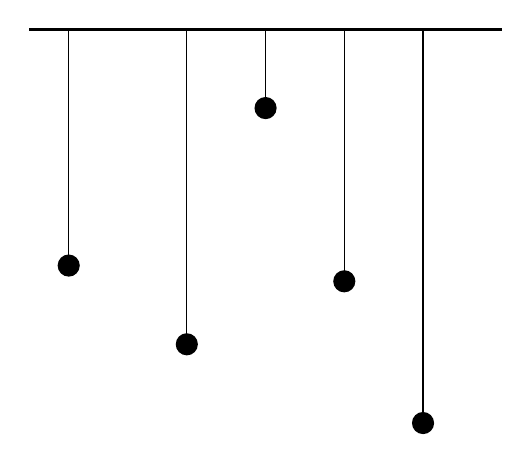
\begin{tikzpicture}
\draw[very thick] (0,0) -- (6,0);
\draw (0.5,0) -- (0.5,-3);
\fill (0.5,-3) circle[radius=4pt];
\draw (2,0) -- (2,-4);
\fill (2,-4) circle[radius=4pt];
\draw (3,0) -- (3,-1);
\fill (3,-1) circle[radius=4pt];
\draw (4,0) -- (4,-3.2);
\fill (4,-3.2) circle[radius=4pt];
\draw (5,0) -- (5,-5);
\fill (5,-5) circle[radius=4pt];
\end{tikzpicture}
\caption{单摆的共振\label{compen}}
\end{figure}
\begin{ans}
共振的条件是频率相等或相近,所以\uline{\hspace{3cm}}。
\end{ans}

\subsection{波动}
波动是某个物理对象在空间中的传播,高中阶段我们只简单研究机械波(振动的传播)和电磁波(电磁场的传播)。
\subsubsection{机械波的传播}
\emph{机械波的图像和简谐振动的图像有什么不同?}
\begin{itemize}
\item
振动是单个质点的独角戏,而波动则是一群质点的群魔共舞。
\item
我们依然只讨论正弦形式的波动。
\item
介质中位置位于$x$处的质点振动 \so 带动介质中附近的其他质点振动 \so 介质中的质点都在做频率相同而相位不同的简谐振动,每个点$x$的位移$y(t,x)$是时间$t$和位置$x$的函数。
\item
给定时间$t$,可以画出一个$y(x)$的图像,称为$t$时刻的波形。
\item
对于振幅不变的波,已知$t_1$时刻的图像,$t_2$时刻的图像可以由$t_1$时刻的图像向前(后)推移$v(t_2-t_1)$实现;$v$称为波速。如\cref{wavediag}。
\cpicn{0.6}{wavediag}{一列以$v=1\unit{m/s}$向右传播的波在不同时刻的波动图像}
\item
机械波的分类:
\begin{enumerate}
\item
横波:位移$y$与波的传播方向垂直,只在固体中存在(原因:只有固体能提供垂直于波速方向的牵引力使得相邻质点垂直于波动方向振动);
\item
纵波:位移$y$与波的传播方向垂直,在固、液、气三态中都能存在。
\end{enumerate}
\item
波动的参数:除了振动的参数$A,\omega,f,T$外,还有波长的波速的概念:波长$\lambda$指$y-x$图上波形的周期,也即介质中两个相位相差$2\pi$的点的距离;波速$v = f\lambda$。
\end{itemize}
\par
\emph{如果只给定两个时刻的波动图像,能确定波的传播方向吗?}
\begin{itemize}
\item
如\cref{wavediag},如果没有指明波向右传播,则波速有很多种可能:
\begin{enumerate}
\item
波向右传播,等价于将$t=0$时刻的波形向右平移$\Delta x$的距离到$t = 0.1\unit s$的波形。那么$\Delta x = 0.1\unit{m} + n\lambda$都可以达到这个效果,于是$v = ( 1+ 10n)\unit{m/s},n=0,1,\dots$;
\item
波向左传播,等价于将$t=0$时刻的波形向左平移$\Delta x$的距离到$t = 0.1\unit s$的波形,那么向左平移$\Delta x = 0.9\unit{m} + n\lambda$都可以达到这个效果,于是$ v = (9+10n)\unit{m/s},n=0,1,\dots$。
\end{enumerate}
\item
综上,波速可以表示为$v = (1+10n)\unit{m/s},n \in {\mathbf Z}$。
\end{itemize}
\par
\emph{平静的水面上放置一皮球,一列水波经过水平位置会不会发生改变?给定一个时刻的波形图,皮球的运动方向如何判断?}
\begin{itemize}
\item
机械波的介质中,各质点都在平衡位置附近简谐振动 \so 质点的$x$坐标不会改变。
\item
质点的速度只能朝$\pm y$方向,具体判断:(1)假设波向波速方向传播一段很小的距离,看质点的位移向上还是向下;(2)风吹草迎坡倒...如\cref{wavevel}。
\cpicn{0.6}{wavevel}{波动图像上质点的运动方向。}
\item
已知质点的运动方向和初始位置,就可以继续画出这个质点做简谐运动的$x-t$图。
\end{itemize}

\subsubsection{电磁波的产生和传播}
\emph{你还记得电磁波家族中的哪些成员?}
\begin{itemize}
\item
如\cref{lccircuit}的电路中会发生震荡,即电流按三角函数周期变化,可以证明$T = 2\pi/\sqrt{LC}$。
\begin{figure}[H]
\centering
\begin{circuitikz}
\draw (0,0) to[short] (2,0) to[L,l=$L$] (2,2) to[short] (0,2) to[C,C=$C$]  (0,0);
\end{circuitikz}
\caption{$LC$震荡电路,一开始$C$充满电\label{lccircuit}}
\end{figure}
\item
开放的$LC$电路可以辐射电磁波;其实任何搭载交流电的导线都可以辐射同频率的电磁波 \so 天线原理。
\item
电磁波的传播:麦克斯韦电磁场理论(其实是著名的麦克斯韦方程组):变化的磁场产生变化的电场(感生电动势对应的物理);变化的电场产生变化的磁场 \so 正弦形式的波动中,$E$和$B$相互激发在空间中传播 \so 电磁波,如\cref{emwave}。电磁波是横波。
\cpicn{0.6}{emwave}{电磁波的传播}
\item
电磁波在真空中传播的速度为光速$c$。麦克斯韦最先从他的理论中算出了电磁波的波速,发现和$c$一致 \so 大胆预测光是一种电磁波(\cref{maxwell})\footnote{一个小冷知识:国际单位制下静电力常量$k$在数值上精确地等于$10^{-7}c^2$,这就和理论上计算的电磁波速度以及安培的定义有关。}。
\cpicn{0.4}{maxwell}{上帝说......,于是就有了光}
\item
电磁波谱:按波长从大到小、频率(也即能量)从小到大:
\beq
\text{无线电波} \to \text{微波} \to \text{红外} \to \text{可见光(红$\to$紫)} \to \text{紫外} \to \text{X射线} \to \gamma\text{射线}
\eeq
可见光的波长大概在几百纳米的量级(计算其频率大概是多少?)。
\end{itemize}

\subsubsection{波的干涉和衍射现象}
\emph{把一个振动音叉的两支前端放在水面上,水面的波纹是怎么样的?如果只有一支放在水面,能看到这样的波形吗?}
\begin{itemize}
\item
波的叠加原理:如果有两列波相遇,则两列波不会互相影响;但介质中每一点的位移是两列波之和。
\item
干涉现象:两列\info{频率相等}的波在空间中某一区域相遇,造成这个空间中某些点的振幅始终加强(相长干涉,constructive)或始终减弱(相消干涉,destructive)的现象。
\item
物理分析:两列波在$x$处的相位差...\so 波峰对波峰;波谷对波谷则相长;波峰对波谷则相消。
\item
惠更斯原理:波在传播的每一点都可以当成新的波源(物理上比较好理解,但数学上太过复杂,甚至涉及到泛函积分...) \so 衍射现象:波穿过小孔或狭缝传播,波长越长,衍射越容易发生。
\item
惠更斯原理可以推出波的反射和折射定律 \so 太复杂所以不考,知道就好(要知道波动光学可以解释光的哪些现象)。
\item
波在不同介质中的传播:波速不同,但频率相同(这一点在高中只能当一个公理记住)\so 波长随之变化,且波长比等于波速比。
\item
波的\info{偏振}:横波只在一个方向振动。
\end{itemize}



\newpage
\section{波动角度下的光学}
我们已经知道光是一种电磁波,因此可以用波动的角度研究光学现象。可以用波动角度解释的光学现象包括直线传播、反射、折射、干涉、衍射和偏振。前三种现象可以用光线模型描述,因此称为几何光学,适用于光的波长远小于物体尺度的情况;干涉和衍射两种现象必须考虑相位差的影响,存在于物体尺度小于波长或与波长相当时,加上偏振现象,相应地被称为波动光学。
\subsection{几何光学}
\emph{如何定量描述折射现象?}
\begin{itemize}
\item
几何光学三大规律:
\begin{enumerate}
\item
光在同种均匀介质中直线传播;
\item
光在镜面上发生反射,反射角等于折射角;
\item
光从一种波速为$v_1$的介质折射到另一种波速为$v_2$的介质时,入射角$i$和折射角$r$服从折射定律
\beq
\frac{\sin i}{\sin r} = \frac{v_1}{v_2}
\eeq
\end{enumerate}
\item
介质的\info{折射率}$n$定义为光速$c$与光在这种介质中的速度$v$的比$n = c/v>1$ \so 从真空(空气)入射到折射率为$n$介质的折射定律
\beq
\frac{\sin i}{\sin r} = n
\eeq
如\cref{refrc}。
\begin{figure}[H]
\centering
\begin{tikzpicture}
\draw (-2,0) -- (2,0) node[right]{界面};
\draw[dotted] (0,2) node[above]{法线} -- (0,-2);
\draw[->] (-2,1.5) -- (-1,0.75);
\draw (-1,0.75) -- (0,0);
\draw[->] (0,0) -- (0.75,-1);
\draw (0.75,-1) -- (1.5,-2);
\draw (0,1) node[above left]{$i$} arc(90:143:1) ;
\draw (0,-1)  node[below right]{$r$} arc(270:307:1);
\end{tikzpicture}
\caption{折射定律\label{refrc}}
\end{figure}
\item
常见值:水的折射率$n = 4/3$;玻璃的折射率$n = \sqrt{3}$(哪里有这么巧...)
\item
全反射:仅在介质$\to$真空(光密$\to$光梳)发生,存在一个\info{临界角度}$C$,使得\info{大于}这个角度的入射光不存在反射光。折射角满足$\sin r = n \sin i <1$ \so $\sin C = \frac{1}{n}$。\so 入射角恰好为$C$时的折射光线平行于界面,如\cref{critical}(光路可逆:平行界面刚好能入射介质的光线折射角为$C$,这样的入射光线称为掠射光)。
\begin{figure}[H]
\centering
\begin{tikzpicture}
\draw (-2,0) -- (2,0) node[right]{界面};
\draw[dotted] (0,2) node[above]{法线} -- (0,-2);
\draw[thick,->] (2,-2) -- (1,-1);
\draw[thick] (1,-1) -- (0,0);
\draw[thick,->] (0,0) --(-1,0);
\draw[thick] (-1,0) -- (-2,0);
\draw[dashed,->] (1.16,-2) node[below]{$a$} -- (0.58,-1);
\draw[dashed] (0.58,-1) -- (0,0);
\draw[dotted,->] (2,-4/3) node[right]{$b$}-- (1,-2/3);
\draw[dotted] (1,-2/3) -- (0,0);
\draw (0,-1) node[below right]{$C$} arc (270:315:1);
\end{tikzpicture}
\caption{全反射\label{critical}}
\end{figure}
\item
想法:入射光线从法线开始向界面逆时针旋转,出射光线也随之逆时针旋转,但旋转更快;到出射光线和法线的夹角为$90^\circ$后,出射光线则无从可去。
\end{itemize}
\begin{eg}
判断\cref{critical}中$a,b$两光线中哪一条发生了全反射?如果$C = 45^\circ$,$a$的入射角为$30^\circ$,求其折射光线的折射角。
\end{eg}
\begin{ans}
\ \\
\ \\
\ \\
\ \\
\end{ans}

\subsection{光的干涉:杨氏双缝}
\emph{你在日常生活中见过哪些光的干涉现象?}
\begin{itemize}
\item
干涉现象必须用波动解释,这也是牛顿早期粒子学说的失败原因。
\item
生活中的干涉现象一般是一束光自身和反射光干涉导致 \so 肥皂泡的薄膜干涉等 \so 过于复杂,高中阶段不深究。
\item
最简单的干涉其实是一个精心设计的实验:杨氏双缝,如\cref{youngs}。
\begin{figure}[H]
\centering
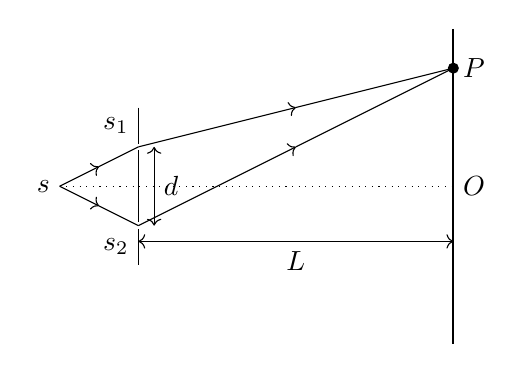
\begin{tikzpicture}
\draw[dotted] (-1,0) node[left]{$s$}-- (4,0) node[right]{$O$};
\draw[->] (-1,0) -- (-0.5,0.25);
\draw (-0.5,0.25) -- (0,0.5);
\draw[->] (-1,0) -- (-0.5,-0.25);
\draw (-0.5,-0.25) -- (0,-0.5);
\draw (0,1) -- (0,0.54) node[above left]{$s_1$};
\draw (0,0.46) -- (0,-0.46);
\draw (0,-0.54) node[below left]{$s_2$}-- (0,-1);
\draw[thick] (4,2) -- (4,-2);
\draw[->] (0,0.5) -- (2,1);
\draw (2,1) -- (4,1.5);
\draw[->] (0,-0.5) -- (2,0.5);
\draw (2,0.5) -- (4,1.5);
\fill (4,1.5) node[right]{$P$} circle[radius=2pt];
\draw[<->] (0,-0.7) -- node[below]{$L$} (4,-0.7);
\draw[<->] (0.2,0.5) -- node[right]{$d$} (0.2,-0.5);
\end{tikzpicture}
\caption{杨氏双缝\label{youngs}}
\end{figure}
\item
经过两缝的光到达屏幕,相位相同则在右侧屏幕上出现明纹;相差$180^\circ$则出现暗纹 \so 路程差为波长整数倍则出现明纹,$\lambda/2$的奇数倍则出现暗纹(原因?回想波动图像前推波形图的原理...)。
\item
Aside: 一个快速估算平方根的小技巧:
\beq
\sqrt{1+x} \approx 1+ \frac{x}{2}, |x|<1
\eeq
例如$\sqrt{2} = \sqrt{1+1} \approx 1.5$;$\sqrt{10} = \sqrt{9\times \lbk 1 + \frac{1}{9}\rbk}  = 3\sqrt{ 1 + \frac{1}{9}} \approx 3 + 1/6$等。更一般的,$(1+x)^\alpha \approx 1+ \alpha x,|x|<1$。(可以从求导的角度理解)
\item
条纹间距公式的推导:记$OP = x$,$s_1 P = \sqrt{L^2 + (x-d/2)^2}$,$s_2 P = \sqrt{L^2 + (x+d/2)^2}$。当$L\gg x,d$时
\bea
s_1 P &\approx L + \frac{ (x-d/2)^2}{2L}, \\
 s_2 P &\approx L + \frac{ (x+d/2)^2}{2L}
 \eea
\so 
\beq
s_2 P - s_1 P = \frac{xd}{L} =
\begin{cases}
 n\lambda &, \text{出现明纹;} \\
\lbk n+\frac{1}{2}\rbk \lambda &,\text{出现暗纹}
\end{cases}
\eeq
 \so 相邻明纹(暗纹)的间距
\beq
\Delta x = \frac{\lambda L}{d}
\eeq
\item
在屏幕中心$O$一定出现明纹。
\item
如果用白光(由很多个不同$\lambda$的光组成),则出现彩色条纹,而没有明显的明暗间隔,且中心$O$一定是白点。
\end{itemize}

\subsection{衍射和偏振}
\emph{电影院里3D眼镜的原理是什么?}
\begin{itemize}
\item
光通过单个狭缝(宽度和波长相当或更小)、或绕过狭小物体传播会发生\info{衍射}现象,在后方的光屏上产生间距不等的条纹(和杨氏双缝区分)。
\item
衍射的典型体现:柏松亮斑、用铅笔芯看日光灯...
\item
偏振是指光的$\vec E$场(或等效地、$\vec B$场)只朝一个方向振动;日常生活中常见的光都是无偏振的(由许多偏振方向随机的光叠加而成)。 \so 偏振片只允许一个方向偏振的光通过 \so 3D电影,左右眼各一个不同方向的偏振片。
\item
反射光是部分偏振光(知道就好)。
\end{itemize}


\newpage
\section{光的波粒二象性和波尔氢原子模型}
\subsection{光电效应}
\emph{在20世纪初发现了两种波动光学无法解释的现象,从而给了物理学家许多创造新理论(i.e. 发论文灌水)的机会。}
\begin{itemize}
\item
\info{康普顿效应}:$X$射线与电子相互作用后,$X$射线的方向和波长发生改变的现象,如\cref{campeff}。
\begin{figure}[H]
\centering
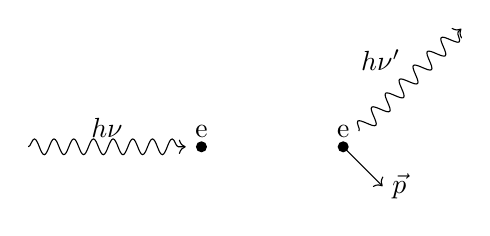
\begin{tikzpicture}
\drawlight{(0,0)}{above}{$h\nu$}{(2,0)}
\fill  (2.2,0) node[above]{e} circle[radius=2pt];
\fill (4,0) node[above]{e} circle[radius=2pt];
\draw[->] (4,0) -- (4.5,-0.5) node[right]{$\vec p$};
\drawlight{(4.2,0.2)}{above left}{$h\nu'$}{(5.5,1.5)}
\end{tikzpicture}
\caption{康普顿效应,电子遇到$X$射线后自身获得一个动量,并且$X$射线的方向和波长改变\label{campeff}}
\end{figure}
\item
\info{光电效应}:光照射到金属(或金属氧化物)板上会\info{立即}发射电子。
\item
由于康普顿效应的数学有一点点复杂,为了降低学习压力我们只研究光电效应。
\item
爱因斯坦1905年用光子学说解释光电效应:光是由一个个光量子(简称光子)构成,对频率为$\nu$\footnote{从此以后我们不再用$f$表示频率,我也不知道为什么。$\nu$是希腊字母,不是$v$,它大概读作niu。}的光,单个光子的能量为$E = h\nu$。
\item
$h = 6.67\times 10^{-34} \unit{J \cdot s}$称为普朗克常数。
\item
光量子最开始由普朗克提出并被他本人抛弃。1905年称为爱因斯坦奇迹年。那一年名不见经传、工作都找不到的爱因斯坦连发4篇论文,其中两篇有关狭义相对论、一篇是光电效应的解释、另一篇关于布朗运动。这4篇文章让他一举成名,并且他凭借对光电效应的解释得了诺贝尔奖(而不是靠相对论)。
\item
光电效应的解释:金属板表面对电子有束缚作用,这个束缚的能量用\info{逸出功}$W$表征;电子会吸收光子的能量$h\nu$,其中一部分用来克服逸出功逃离金属表面,剩下的部分转换成电子的动能$E_k = h\nu - W$。
\item
探究光电效应的实验电路图(简化版)如\cref{pecir}。
\begin{figure}[H]
\centering
\begin{circuitikz}[american]
\draw  (0,0) to[short] (0,2) to[C] (4,2) to[short] (4,1.35) ;
\draw (0,0) to[vsource,v=$U$] (4,0);
\draw (4,0.65) to[short] (4,0);
\draw (4,1) node{A} circle[radius=0.35];
\draw (2,2) circle[radius=0.7];
\drawlight{(0.8,3.2)}{above right}{$h\nu$}{(1.5,2.7)}
\drawlight{(0.6,2.9)}{above}{}{(1.2,2.4)}
\draw[->] (3.5,0.5) --node[left]{$I$} (3.5,1.5);
\end{circuitikz}
\caption{光电效应的电路图\label{pecir}}
\end{figure}
\item
\cref{pecir}中$U$是一个可调电压源(可以用一个分压电路具体实现),电子从左向右流动、和电流流动方向相反。阴极(左边迎光极板,发射电子)电压高于右边阳极,相应电子在阴极的势能低于阳极,电子从左到右需要克服电场力做功$eU$。
\item
阴极发射电子$E_k = h\nu - W$;如果调节$U$使得电子能够刚好从阴极$\to$阳极,动能定理
\beq
0 - E_k = -eU
\eeq
联立两式得
\beq
eU = h\nu - W
\eeq
\item
截止电压$U_e = \frac{h\nu -W}{e}$。电源电压高于这个电压则不会发生光电效应。$U_e$只和光的频率、阴极性质有关;和光强无关(光强$\approx$光子数)。
\item
画$U_e - \nu$的图像,斜率为$h/e$ \so 测量普朗克常数$h$。
\item
固定$\nu$画$I-U$的图像(这个时候一般喜欢把电源反过来,让$I$随$U$增大),存在一个饱和电流$I_S$和光强有关(物理理解:光子数越多,打出来的电子越多),如\cref{sati}。
\cpicn{0.5}{sati}{不同光强下的$I-U$曲线}
\end{itemize}

\subsection{原子结构}
\emph{从初中到现在,你对原子内部结构的认识有变化吗?}
\begin{itemize}
\item
汤普森枣糕模型 \so 卢瑟福太阳系模型 \so 波尔氢原子 \so 电子云模型 \so ???
\item
卢瑟福用$\alpha$粒子轰击金箔(几个原子层厚度)发现
\begin{enumerate}
\item
大多数粒子近乎径直穿过金箔;
\item
少数粒子发生小角度偏移;
\item
极少数粒子被反弹。
\end{enumerate}
\so 原子几乎是空的,原子核在原子中心一个很小的区域,原子核带正电(分别对应哪一条实验现象?)
\item
无法解释电子自发辐射问题 \so 学生波尔提出波尔模型:电子轨道量子化。
\item
只对氢原子适用:电子绕原子核旋转,库仑力提供圆周运动的向心加速度
\beq
\frac{ke^2}{r^2} = \frac{mv^2}{r} \quad \Rightarrow \quad r = \frac{ke^2}{mv^2}
\eeq
\item
看似任意的$r$,波尔要求,仅有$mvr = n \frac{h}{2\pi}$的轨道是稳定的 \so $r = \frac{(h/2\pi)^2 n^2}{mke^2} \propto n^2$
\item
每一个$r$对应一个能量(动能+势能)$E = -\frac{ke^2}{2r}$ \so 能量也是量子化的,$E \propto \frac{1}{n^2}$。
\item
所谓\info{量子化}是指某一物理量只能去离散的分立值,例如电荷量$q$就是以$e$为单位量子化的。量子化的能量称为\info{能级}。
\item
最低能量对应$n=1$,对应的半径称为波尔半径$a_0 = 0.053\unit{nm}$;能量称为里德堡能量$E_1 = -13.6\unit{eV}$。\so 第$n$能级的半径和能量
\bea
r_n &= n^2 a_0;\\
E_n &= \frac{-13.6}{n^2} \unit{eV}
\eea
示意图如\cref{bohrorbit}。
\begin{figure}[H]
\centering
\begin{tikzpicture}
\draw (0,0) node{$+$} circle[radius = 5pt];
\draw[dotted] (0,0) circle[radius = 0.5] ;
\node at(0,0.5) {$-13.6\unit{eV}$};
\draw[dotted] (0,0) circle[radius = 2] ;
\node at(2,0) {$-3.4\unit{eV}$};
\draw[dotted] (0,0) circle[radius = 4.5] ;
\node at(4.5,0){$-1.51\unit{eV}$};
\end{tikzpicture}
\caption{波尔氢原子的轨道量子化\label{bohrorbit}}
\end{figure}
\item
原子结构的现代观点(其实也不是特别现代...):电子云,电子在原子核周围按一定的概率密度出现。
\end{itemize}

\subsection{波尔氢原子中的能级跃迁}
\emph{焰色反应的原理是什么?}
\begin{itemize}
\item
$n=1$的电子称为\info{基态},能量最低;$n>1$则是\info{激发态}。激发态不稳定,可以发出光子跃迁到能量较低的态 \so 光子能量满足$h\nu = E_m - E_n, m>n$。电子也可以吸收光子或加热被激发,跃迁到高能量的态(焰色反应的原理)。
\item
能级图表示跃迁,如\cref{bohrlevel}。
\begin{figure}[H]
\centering
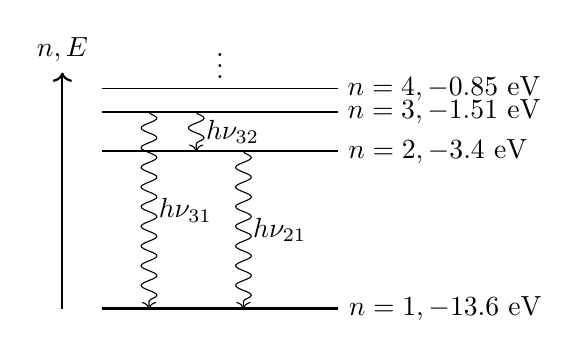
\begin{tikzpicture}
\draw[->,thick] (-0.5,0) -- (-0.5,3) node[above]{$n,E$};
\draw[very thick] (0,0) -- (3,0) node[right]{$n=1,-13.6\unit{eV}$};
\draw[thick] (0,2) -- (3,2) node[right]{$n=2,-3.4\unit{eV}$};
\draw(0,2.5) -- (3,2.5) node[right]{$n=3,-1.51\unit{eV}$};
\draw[thin] (0,2.8) -- node[above]{$\vdots$} (3,2.8) node[right]{$n=4,-0.85\unit{eV}$};
\drawlight{(0.6,2.5)}{right}{$h\nu_{31}$}{(0.6,0)}
\drawlight{(1.2,2.5)}{right}{$h\nu_{32}$}{(1.2,2)}
\drawlight{(1.8,2)}{right}{$h\nu_{21}$}{(1.8,0)}
\end{tikzpicture}
\caption{波尔氢原子的能级图\label{bohrlevel}}
\end{figure}
\item
一个非常有用的单位组合:$hc = 1240\unit{eV\cdot nm}$。
\item
跃迁可以一步到位,也可以分步进行 \so 位于第$n$能级的电子向基态($n=1$)跃迁可以产生${\rm C}^2_{n-1}$种波长的光。
\item
从$n\to m$能级跃迁产生光的波长:由
\beq
\begin{cases}
h\nu_{nm} &=E_n - E_m =  -|E_1| \lbk \frac{1}{n^2} - \frac{1}{m^2}\rbk;\\
\nu_{nm}\lambda_{nm} &= c.
\end{cases}
\Rightarrow  \frac{1}{\lambda_{nm}} =\frac{hc}{|E_1|} \lbk \frac{1}{m^2} - \frac{1}{n^2}\rbk
\eeq
\end{itemize}
\newpage
\section{狭义相对论与原子核}
\subsection{狭义相对论}
\emph{怎么理解$E=mc^2$?}
\begin{itemize}
\item
速度接近光速时,狭义相对论的三大经典现象:尺缩、钟慢、动质量(知道就好,不用深究,像动质量这种观点现在看来也是不准确的)。
\item
狭义相对论的基本原理:光速不变,且所有惯性参考系等价。
\item
速度的洛伦兹变换$v' = (u+v)/(1-uv/c^2)$保证了不能通过速度叠加的方式超光速。
\item
质能关系$E = mc^2$的理解:事实上表明了质量也是一种能量,加上质量,宇宙的总能量还是守恒的。例如一个粒子$A$衰变成两个$B$粒子,但实验发现$2m_B < m_A$ \so 加上质量的能量守恒,这个缺失的质能$(m_A - 2m_B)c^2$必定转化为其他形式的能量,例如$B$粒子的动能或反应中放出的其他粒子(比如光子、中微子)中的能量。
\end{itemize}
\begin{eg}
一个静止的粒子A衰变成两个B粒子,但实验发现$2m_B < m_A$。若衰变过程中没有其他粒子放出,且$B$粒子的速度远小于光速,求反应后两个$B$粒子的速度。
\end{eg}
\begin{ans}
根据能量守恒和质能关系,设两个$B$粒子的速度分别为$v_1$和$v_2$,有
\beq
m_A c^2 = 2m_B c^2 + \frac{1}{2} m_B v_1^2 + \frac{1}{2} m_B v_2^2
\eeq
再由于初始时刻系统动量为零,由动量守恒
\beq
0=m_B v_1 + m_B v_2
\eeq
解得
\beq
v_1 = -v_2 = \sqrt{\frac{m_A - 2m_B}{m_B}} c
\eeq
\end{ans}

\subsection{原子核的构成}
\emph{恒星的能源主要来源于核聚变。当恒星的氢全部聚变成了氦后,变会继续发生${\rm He \to Be}$等聚变过程。但观测发现这个聚变过程到${\rm Fe}$就截止了,为什么会这样?}
\begin{itemize}
\item
查理维克最先发现了中子 \so 后人提出原子核模型,由中子(n,不带电)和质子(p,带正电$+e$)构成。$m_p \approx m_n \gg m_e$。
\item
原子核的表示为$^A_Z{\rm X}$,$A$为质量数、$Z$为质子数、${\rm X}$为元素符号(复习化学知识)。
\item
中子和质子统称为核子。核子间存在电磁相互作用和强相互作用。这些相互作用都具有对应的势能,从而将一堆核子从远处聚集在一起形成原子核${\rm X}$时会发生质量亏损:核子之间形成原子核的状态是束缚态,类似电子-质子形成的束缚态,其能量为$-E_B(A,Z)$,为一负数;实际测到的核质量满足
\beq
Zm_pc^2 + (A-Z)m_n c^2- E_B(A,Z) = m_{\rm X}c^2 
\eeq
\item
因此核的质量小于构成它们的核子的质量,$E_B$称为结合能,一般都随$A$增大而增大。
\item
每个核子的平均结合能$\frac{E_B}{A}$称为\info{比结合能},比结合能越大、核子越稳定。比结合能曲线$\frac{E_B}{A} - A$在铁核附近达到最大值 \so 铁是(在核物理意义上)最稳定的元素。
\item
进一步深入,把核子也拆开 \so 粒子物理标准模型:核子由3个夸克构成。粒子物理标准模型中有包括夸克内的下面成员:
\begin{enumerate}
\item
夸克:一共有6(正粒子)+6(反粒子)种,构成核子和其他一些质量非常大的奇异粒子,参与所有相互作用;
\item
轻子:轻子不参与强相互作用,包括电子e、$\mu$子、$\tau$子和对应的三种中微子,以及这6种粒子的反粒子,它们的质量很轻,中微子的质量几乎为零;
\item
波色子:包括光子、胶子和中间波色子(Z和W),分别传递电磁、强和弱相互作用。还有一个赋予其他粒子质量的希格斯波色子。波色子没有反粒子。
\end{enumerate}
\emph{
粒子物理标准模型在上世纪末由一系列理论和实验物理学家建立起来,可以说是理论物理在上世纪末的最伟大成就。杨振宁和他当时的学生米尔斯建立了规范场论(也称杨-米尔斯理论),将电磁、强、弱三种基本相互作用的描述统一在一个数学框架下!}
\end{itemize}

\subsection{核反应}
\emph{为什么核反应方程式左边的反应物不会超过2个?}
\begin{itemize}
\item
一般来说核反应可以放出巨大的能量:一般化学反应放出称能量是${\rm eV}$量级(对应氢原子能级的能量);核反应可以达到${\rm keV} - {\rm MeV}$量级(对应核子的质量)。$1\unit{MeV} = 10^6 \unit{eV}$。
\item
核子质量用原子质量单位${\rm u}$,使得${\rm n,p}$的质量都大概是$1\unit u$;也常用${\rm MeV}/c^2$作单位,$1\unit{u} = 931.5\unit{MeV}/c^2$。
\item
核反应一般表达式:用原子核符号和$\to$表示,其他类似化学方程式。
\item
核反应满足的守恒定律:
\begin{enumerate}
\item
能量守恒和动量守恒:能量包括各个粒子的$mc^2$;
\item
电荷守恒;
\item
质量数守恒(即核子数守恒;反质子的核子数为$-1$)。
\end{enumerate}
如果考虑轻子参与反应,则轻子数也应该守恒(反粒子的轻子数为$-1$,了解即可)。
\item
核反应包括\info{衰变}和\info{聚变}。
\item
聚变是轻核$\to$重核,到铁之前到聚变反应都是放能的,但需要高温环境(e.g. 恒星中心温度)。
\item
衰变是重核$\to$轻核,包括$\alpha,\beta,\gamma$三种,特点如\cref{decaytab}。
\begin{table}[H]
\centering
\begin{tabular}{c|c|c}
衰变类型 & 核反应通式 & 实质 \\ \hline
$\alpha$衰变 & $^A_Z {\rm X} \to ^{A-4}_{Z-2} {\rm X} + ^4_2{\rm He}$ & -- \\ \hline
$\beta$衰变 & $^A_Z {\rm X} \to ^{A}_{Z+1} {\rm X} + {\rm e}^-$  & 中子衰变:${\rm n} \to {\rm p} +{\rm e}^- +\bar{\nu}_e$  \\ \hline
$\gamma$衰变 & ${\rm X}^* \to {\rm X} + \gamma$ & 处于激发态的原子或原子核放出高能光子 \\
\end{tabular}
\caption{三种衰变\label{decaytab}}
\end{table}
\item
自发衰变存在半衰期$T$,为原核素减少一半的时间,几乎与核所处的环境(温度、是否形成化合物等)无关 \so 经过$nT$时间后原核素剩下$\lbk \frac{1}{2}\rbk^{n}$。
\item
裂变是用中子轰击重核,重核物质超过临界体积可以发生链式反应使得裂变反应雪崩式发生 \so 核弹
\item
高中物理到最后可以说是越来越简单...学到后面连个像样的公式都没有了,主要是因为这些东西深究起来太过复杂,数学要求远远超过了小学水平(可能也超过了目前人类的计算水平)。
\end{itemize}
\begin{eg}
磁场中一个静止的核($Z>4$)发生$\alpha$衰变,两种衰变产物在磁场中的轨迹半径分别为$R_1$和$R_2$,求$R_1:R_2$。
\end{eg}
\begin{ans}
动量为$p$的带电粒子在磁场中的轨道半径可以表示为$R = \frac{p}{qB}$。\vspace{2cm}
\end{ans}













\end{document}